Un vidrier està reparant un dels vitralls de la Sagrada Família, la forma del qual és la de la part ombrejada
de la figura adjunta. S'ha adonat que Gaudí el va dissenyar de manera que un dels costats segueix la funció
$y=3\sin(x/4)$ i un altre segueix la funció $y=3\cos(x/4)$, on $x$ i $y$ estan expressades en metres.
\begin{center}
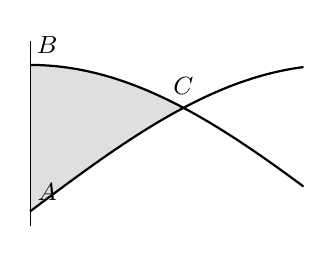
\begin{tikzpicture}[x=0.62cm,y=0.62cm]
  \fill[gray!25] plot[domain=0:3.14159,samples=40,smooth] (\x,{3*sin(\x/4 r)})
    -- plot[domain=3.14159:0,samples=40,smooth] (\x,{3*cos(\x/4 r)}) -- cycle;
  \draw (0,-0.3) -- (0,3.5);
  \draw[\colorgrafica,thick] plot[domain=0:5.6,samples=60,smooth] (\x,{3*sin(\x/4 r)});
  \draw[\colorgrafica,thick] plot[domain=0:5.6,samples=60,smooth] (\x,{3*cos(\x/4 r)});
  \node[font=\small] at (0.35,3.4) {$B$};
  \node[font=\small] at (0.35,0.4) {$A$};
  \node[above,font=\small] at (3.14159,2.2) {$C$};
\end{tikzpicture}
\end{center}

\begin{apartats}

\apartat{1}
Raoneu a quina funció correspon cada gràfica i calculeu les coordenades dels punts $B$ i $C$ assenyalats a la
figura (tenint en compte que $A$ és l'origen de coordenades).

\begin{solucio}
Com que $3\sin\left(\frac04\right)=0$ i $3\cos\left(\frac04\right)=3$, la gràfica inferior (la que passa pels
punts $A$ i $C$) és la del sinus, i la superior (la que passa per $B$ i $C$) és la del cosinus. El punt $B$
correspon al valor $3\cos\left(\frac04\right)=3$; per tant, és el punt $B=(0,3)$. Finalment, el punt $C$ és el
punt de tall entre el sinus i el cosinus, $3\sin\left(\frac x4\right)=3\cos\left(\frac x4\right)$:
\[
\frac{3\sin\left(\frac x4\right)}{3\cos\left(\frac x4\right)}=1\;\rightarrow\;\tan\left(\frac x4\right)=1
\;\rightarrow\;\frac x4=\frac\pi4\;\rightarrow\;x=\pi .
\]
Com que $3\sin\left(\frac\pi4\right)=3\cos\left(\frac\pi4\right)=\frac{3\sqrt2}{2}$, el punt de tall és
$C=\left(\pi,\frac{3\sqrt2}{2}\right)$.

\textit{Pauta oficial:} 0,5 per raonar quina gràfica és cadascuna; 0,25 per les coordenades del punt $B$, i
0,25 per les de $C$.
\end{solucio}

\apartat{1,5}
Calculeu el preu del vitrall sabent que costa $750\ \text{€}/\text{m}^2$.

\begin{solucio}
Per a calcular el preu del vitrall, necessitem trobar la seva àrea:
\begin{align*}
A&=\int_0^\pi\left(3\cos\left(\frac x4\right)-3\sin\left(\frac x4\right)\right)dx
=\left[12\sin\left(\frac x4\right)+12\cos\left(\frac x4\right)\right]_0^\pi\\
&=12\left(\sin\left(\frac\pi4\right)+\cos\left(\frac\pi4\right)-\sin(0)-\cos(0)\right)
=12\left(\frac{\sqrt2}{2}+\frac{\sqrt2}{2}-0-1\right)=12\left(\sqrt2-1\right)\simeq4{,}97\ \text{m}^2 .
\end{align*}
Per tant, el preu del vitrall serà de $4{,}97\ \text{m}^2\cdot750\ \text{€}/\text{m}^2=3\,727{,}5$ €.

\textit{Pauta oficial:} 0,25 per plantejar la integral correctament; 0,5 per la primitiva; 0,5 per trobar
l'àrea, i 0,25 pel preu final. Compteu 0 de la part de la primitiva si no tracten adequadament el coeficient
del sinus i del cosinus.

\textit{Nota del banc:} el criteri oficial hi escriu $4{,}97\cdot750=3\,725{,}5$ €, però
$4{,}97\cdot750=3\,727{,}5$. El valor exacte és $12\left(\sqrt2-1\right)\cdot750=9\,000\left(\sqrt2-1\right)\approx3\,727{,}92$ €.
\end{solucio}

\end{apartats}
